\chapter{Data Acquisition \& Management}

%-Discuss the importance of data acquisition and management systems.

\section{Data Acquisition Infrastructure}

%-Explain the general approach pursued in this thesis.

\section{Data Management Requirements}

%-List some requierement for scientific data management.

\section{PyView}

%-Discuss the philosophy of PyView

\subsection{Overview}

\begin{figure}[ht!]
	\centering
	\includegraphics[width=\textwidth]{"./material/figures/appendix/data-acquisition/pyview_schematic"}
	\caption[]{}
	\label{fig:pyview_schematic}
\end{figure}

%-Give an overview of all system components.

\subsection{Instrument Management}

%-Discuss the creation and interfacing of instruments and the management of parameters.


\begin{SCfigure}[1.0][ht!]
	\centering
	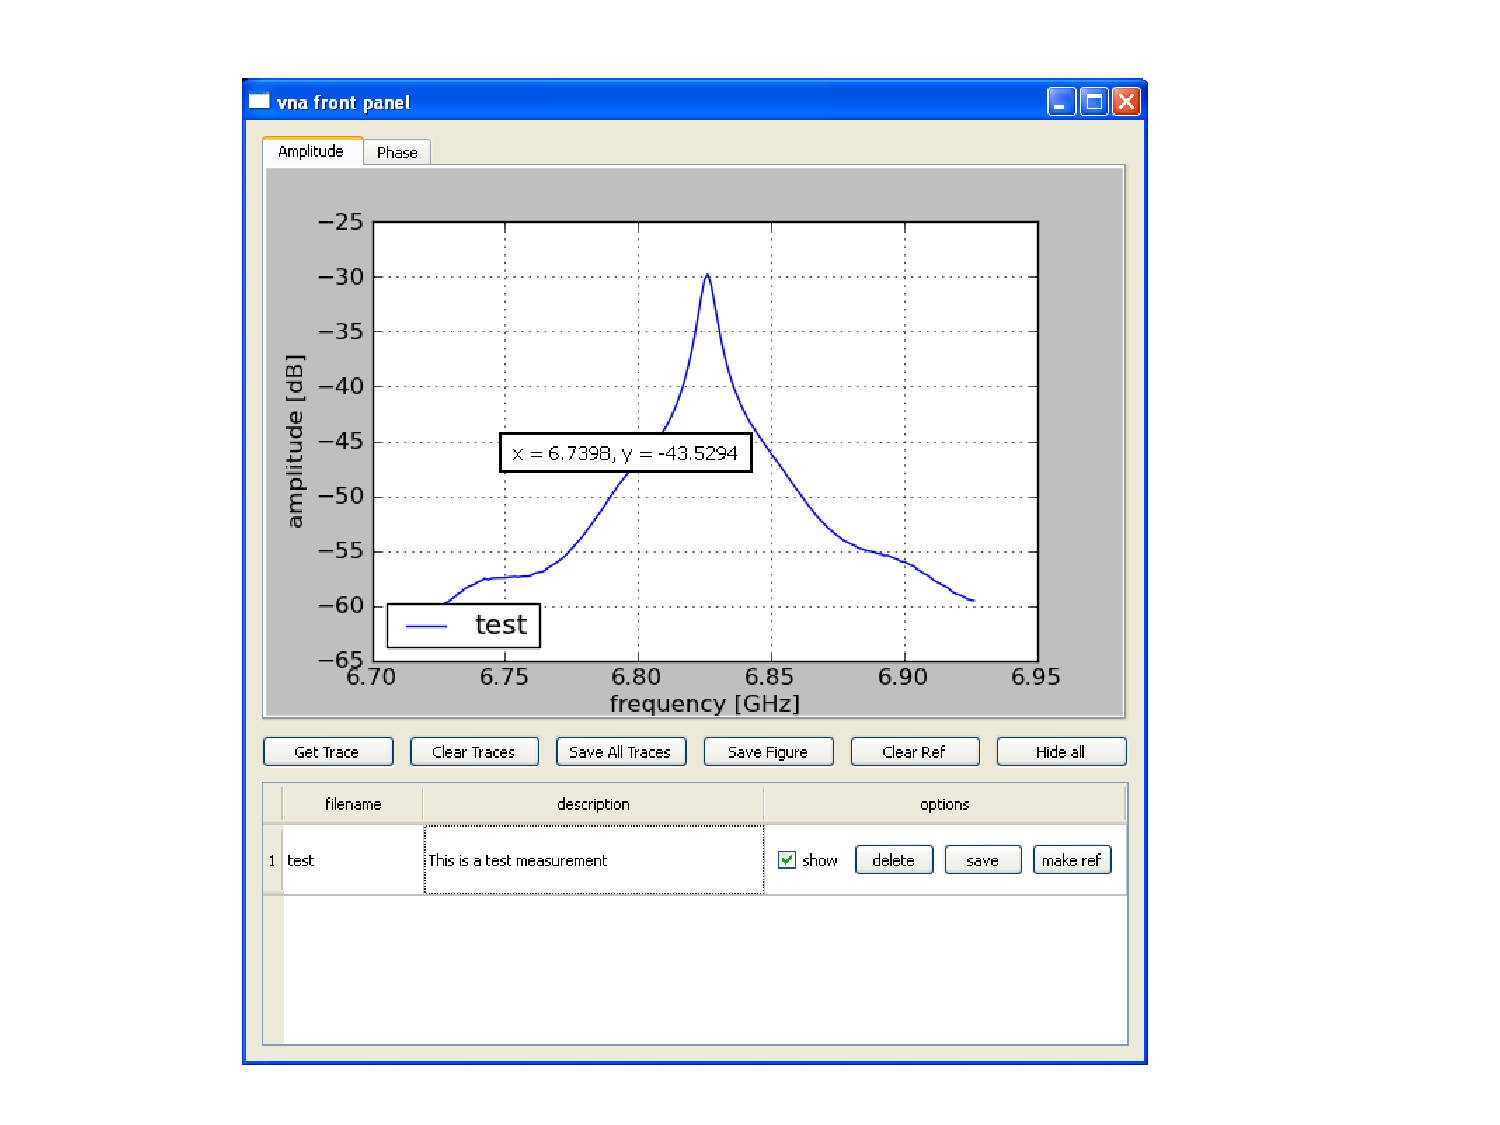
\includegraphics[width=0.5\textwidth]{./material_thesis/python_frontpanel}
	\caption[]{}
	\label{fig:python_frontpanel}
\end{SCfigure}

\subsection{Data Acquisition}

%-Discuss the data acquisition process

\subsection{Data Management}

%-Discuss the data management capabilities of the system.

\subsection{Integrated Data Acquisition \& Analysis}

%-Discuss the data analysis functions of the software.

\begin{figure}[ht!]
	\centering
	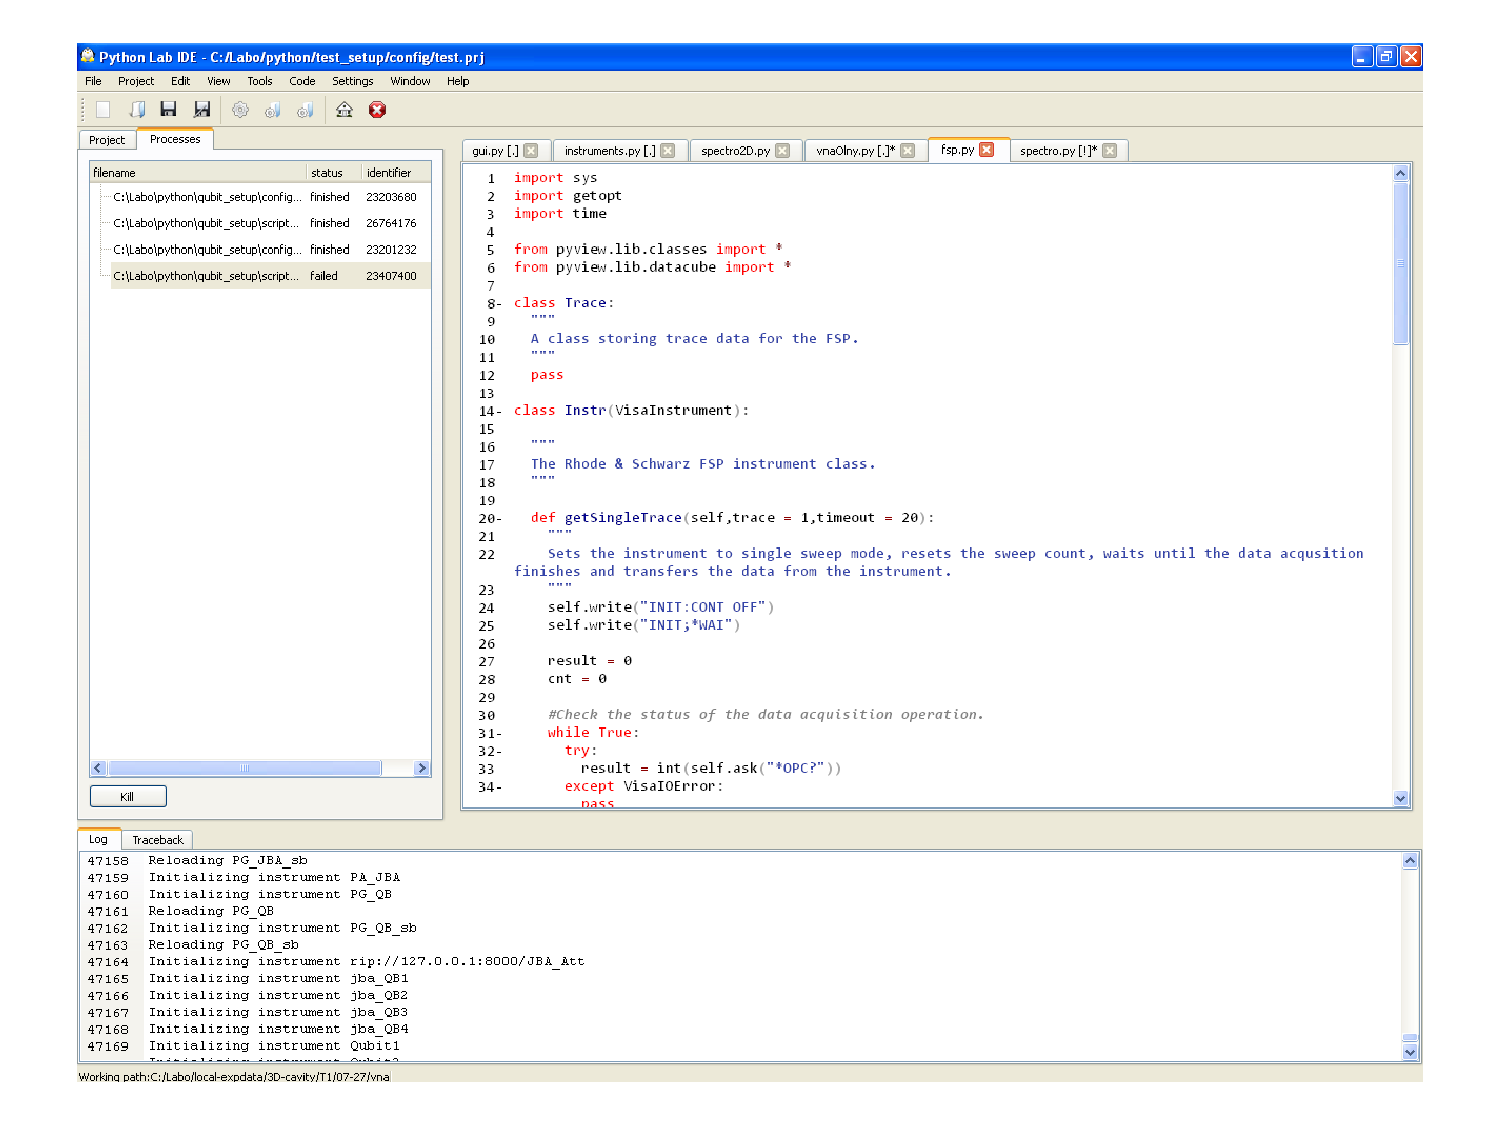
\includegraphics[width=\textwidth]{./material_thesis/python_lab_ide}
	\caption[]{}
	\label{fig:python_ide}
\end{figure}